\documentclass[12pt,a4paper]{article}
\usepackage[top=2.7cm, bottom=2cm, left=2cm, right=2cm]{geometry}
\usepackage[utf8]{inputenc}
\usepackage{CJKutf8}
\usepackage{enumitem}
\usepackage{verbatim}


%% Useful packages
\usepackage{amsmath,amssymb}
% \usepackage{subfigure}
\usepackage{graphicx,wrapfig}
\usepackage[dvipsnames,table]{xcolor}
\usepackage[table]{xcolor}
\usepackage{url}
\usepackage{setspace}
\usepackage[colorlinks=true,anchorcolor=black,linkcolor=Blue,urlcolor=RoyalBlue]{hyperref}
\usepackage[linesnumbered,ruled,vlined]{algorithm2e}
\usepackage{threeparttable}

\usepackage{tikz}
\usepackage{blindtext}
\usepackage{titlesec}
\usepackage{courier}
\usepackage{pdfpages}

\usepackage{lastpage}
\usepackage{fancyhdr}
\setlength{\headheight}{0pt}
\renewcommand{\headrulewidth}{1pt} % remove lines
\renewcommand{\footrulewidth}{0pt}
\pagestyle{fancyplain}
\fancyhf{}
\lhead{
  \textcolor{Gray}{Group 2}
}
\rhead{
  \begin{CJK}{UTF8}{bkai}
  \textcolor{Gray}{實驗物理學實驗結報}
  \end{CJK}
}
\lfoot{
   \textcolor{Gray}{March 11}
  }
\rfoot{
  \thepage/\pageref{LastPage}
  }

\title{\vspace{-0.5cm}
       {\bf \textcolor{black}{{\LARGE 
       \begin{CJK}{UTF8}{bkai}
       實驗物理學(二)\\
       \vspace{6pt}
       實驗結報\\
       \vspace{60pt}
       實驗三、運算放大器\\
       \vspace{6pt}
       Operational Amplifier
       \end{CJK}
       }}
       }
       }
\author{}
\date{}

\begin{document}
\begin{CJK}{UTF8}{bkai}

\maketitle
\thispagestyle{empty}

\vspace{10cm}
\begin{center}
{\large 第二組}\\ \vspace{12pt}
{\large \makebox[3em][s]{洪\hspace{\fill}瑜} B125090009}\\ \vspace{6pt}
{\large \makebox[3em][s]{黃巧涵}  B122030003}\\ \vspace{6pt}
{\large \makebox[3em][s]{洪懌平} B102030019}\\ \vspace{12pt}
{\large 2025/03/11}\\
\end{center}

\clearpage

\vspace{1cm}
\begin{center}
{\large\bf\sc 摘要}
\end{center}

\noindent 

此次實驗研究主題為運算放大器(型號:UA741) ,使用電源供應器、訊號產生器及麵包板等器材搭建反相放大器(Inverting Amplifier)、同相放大器(Non-inverting Amplifier)及隨耦器(Voltage Follower, Buffer Amplifier),並以示波器紀錄經運算放大器產生之波型。 

\section{前言}
\hfill

本實驗的主要目標是探討運算放大器的基本應用,我們將透過實驗驗證反相放大器(Inverting Amplifier)、同相放大器(Non-inverting Amplifier)及隨耦器(Voltage Follower, Buffer Amplifier)的特性與行為。 

In the following subsections, we will introduce the principles utilized in these experiments.

\subsection{運算放大器 (Operational Amplifier or Op-Amp)}
\hfill

是一種電子元件,主要用於放大輸入訊號。它有極高的增益(gain),可以將微弱的電 壓訊號放大到所需的水平。運典型的運算放大器電路有兩個輸入端(反相輸入端−和非反相輸入端+)以及一個輸出端。可以利用外接電阻或電容的方式使放大器有不同的形式,如同相放大器、反相放大器、比較器及電壓跟隨器等等。 

\begin{figure}[h]
    \centering
    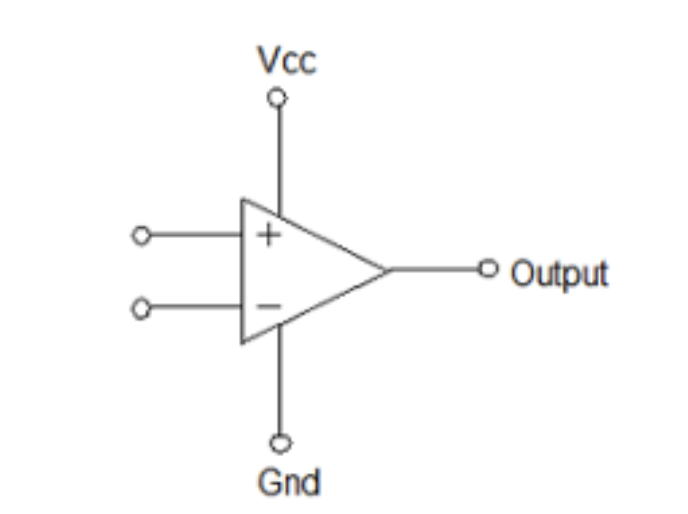
\includegraphics[width=0.5\linewidth]{figures/opamp.png}
    \caption{運算放大器電路示意圖}
    \label{fig:opamp}
\end{figure}

Fig.\ref{fig:opamp}為放大器的簡易連接,運算放大器會將兩個輸入端之電壓差值乘以其增益量,而因增益量很高,需在輸出到輸入間連接電阻降低增益。 

\subsection{同相放大器}
\hfill

Fig.\ref{fig:noninvert}為同相放大器之電路,此為非反相輸入接收訊號,而反相輸入連接在 $R_2$和$R_1$之間。當輸入訊號為正或負移動時,輸出會保持同相,並保持反相輸入端的電壓與同相輸入端之電壓相同。


\begin{figure}[h]
    \centering
    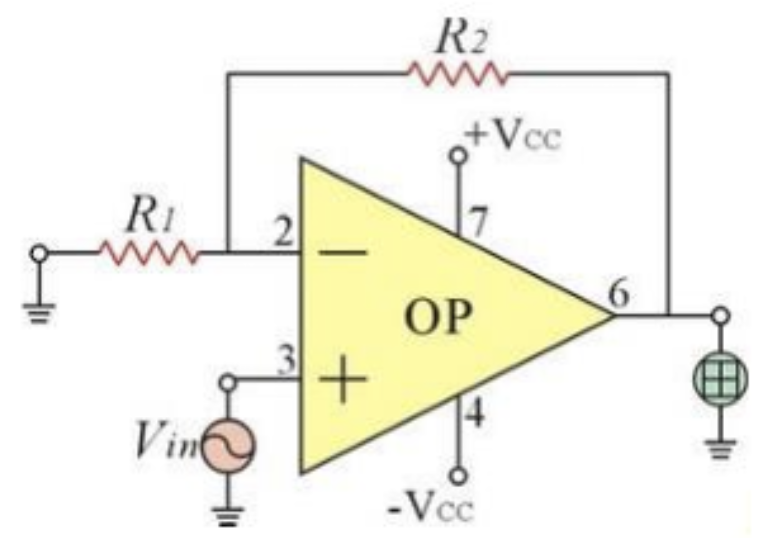
\includegraphics[width=0.4\linewidth]{figures/noninvert.png}
    \caption{同向放大器電路示意圖}
    \label{fig:noninvert}
\end{figure}

本實驗之結構概念:
\begin{enumerate}
    \item 輸入電壓($V_{in}$)連接到非反相輸入端(標記為+端),即第3腳
    \item 反相輸入端(標記為-端,腳位2)通過電$R_1$接地,並透過電阻$R_2$與輸出$V_{out}$連接(第6腳)
\end{enumerate}

公式推導:
\begin{itemize}
    \item 由於運算放大器的增益非常高,並且電路中使用了負回授,根據「虛短」的特性,可以認為反相$V_-$的電壓接近於非反相端的電壓。因此
    \begin{equation}
        V_-\approx V_+ = V_{in}
    \end{equation}
    根據電壓分壓原理,得
    \begin{equation}
        V_-=V_{in}=\frac{R_1}{R_1+R_2}V_{out}
    \end{equation}
    i.e.,
    \begin{equation}
    \label{eq:noninvert}
        V_{out} = V_{in}\left(1+\frac{R_2}{R_1}\right)
    \end{equation}
    \item 增益定義:
    \begin{equation}
        A=\frac{V_{out}}{V_{in}}
    \end{equation}
    再承Eq.\ref{eq:noninvert},得:
    \begin{equation}
        A=1+\frac{R_2}{R_1}
    \end{equation}
\end{itemize}

\subsection{反向放大器}
\hfill

Fig.\ref{fig:invert}為反相放大器之電路,由$R_1$輸入訊號,$R_2$將輸出返回到反相輸入;而若輸入訊號為正,輸出訊號為負,反之亦然。輸出相對於輸入之電壓變化取決於電阻$R_1$和$R_2$的比率。 

\begin{figure}[h]
    \centering
    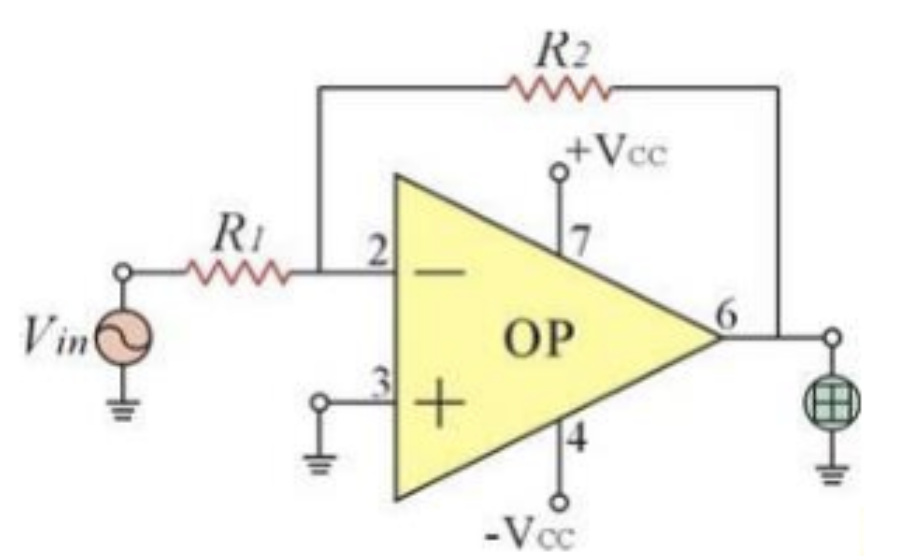
\includegraphics[width=0.5\linewidth]{figures/invert.png}
    \caption{反向放大器電路示意圖}
    \label{fig:invert}
\end{figure}


本實驗之結構概念:
\begin{enumerate}
    \item 輸入電壓($V_{in}$)經過電阻$R_1$接到反相輸入端(標記為-端,即第2腳)
    \item 非反相輸入端(標記為+端,腳位3)接地
    \item 反相輸入端透過電阻$R_2$與輸出端$V_{out}$相連(第6腳)
\end{enumerate}
% \clearpage
公式推導:
\begin{itemize}
    \item 由於運算放大器的增益非常高,並且電路中使用了負回授,根據「虛短」的特性,運算放大器會自動調整輸出電壓,使得反相輸入端的電壓
    \begin{equation}
        V_-\approx V_+ =0
    \end{equation}
    因為$V_+$接地。由於理想運算放大器的輸入阻抗無窮大,所以反相輸入端$V_-$節點的輸入電流可以忽略不計,因此流經$R_1$的電流$I_1$會等於$R_2$的電流$I_2$,使用柯希荷夫電路定律寫出以下表達式:
    \begin{equation}
        \frac{V_{-}-V_{in}}{R_1} = \frac{V_{out}}{R_{2}}
    \end{equation}
    i.e.,
    \begin{equation}
        \frac{V_{in}}{R_1} = -\frac{V_{out}}{R_2}
    \end{equation}
    得出$V_{out}$:
    \begin{equation}
    \label{eq:invert}
        V_{out} = -V_{in}\frac{R_2}{R_1}
    \end{equation}
    
    \item 增益定義:
    \begin{equation}
        A=\frac{V_{out}}{V_{in}}
    \end{equation}
    再承Eq.\ref{eq:invert},得:
    \begin{equation}
        A=1+\frac{R_2}{R_1}
    \end{equation}
\end{itemize}

\subsection{隨耦器}
\hfill

\begin{figure}[h]
    \centering
    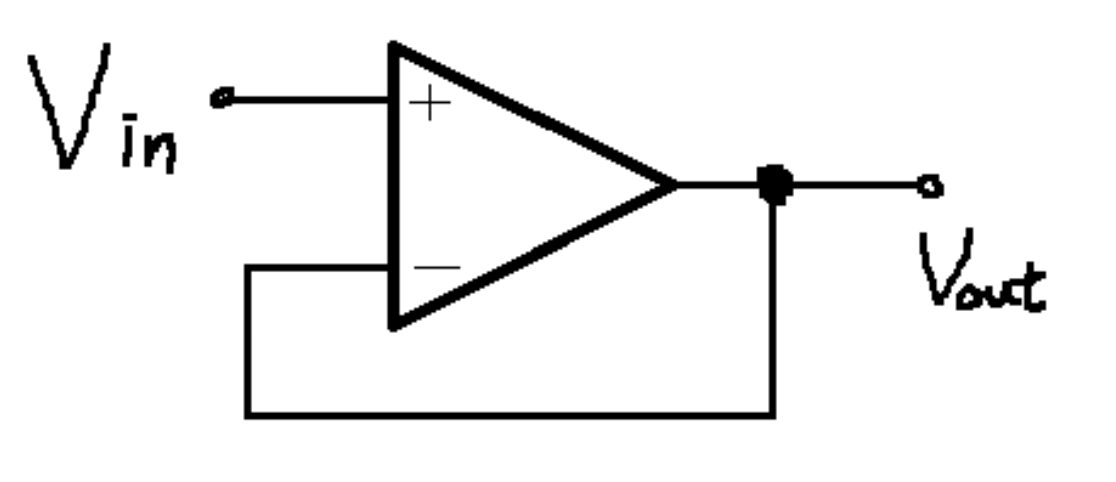
\includegraphics[width=0.5\linewidth]{figures/follower.png}
    \caption{隨耦器電路示意圖}
    \label{fig:follower}
\end{figure}

Fig.\ref{fig:follower}為隨耦器之簡易電路圖,其為一種增益接近1,但具有高輸入阻抗和低輸出阻抗的放大電路;緩衝放大器的輸入與輸出訊號波形相似,但可能會有輕微的相移,主要由於頻率響應、內部電容與寄生電容效應影響。這些因素在高頻時會導致輸出訊號相較輸入訊號略微滯後。


\clearpage
\section{實驗步驟和紀錄}

\subsection{反向放大器}\label{subsec:step_1}
\hfill


\begin{enumerate}
    \item 連接電路如Fig.\ref{fig:invert}
    \begin{figure}[h]
        \centering
        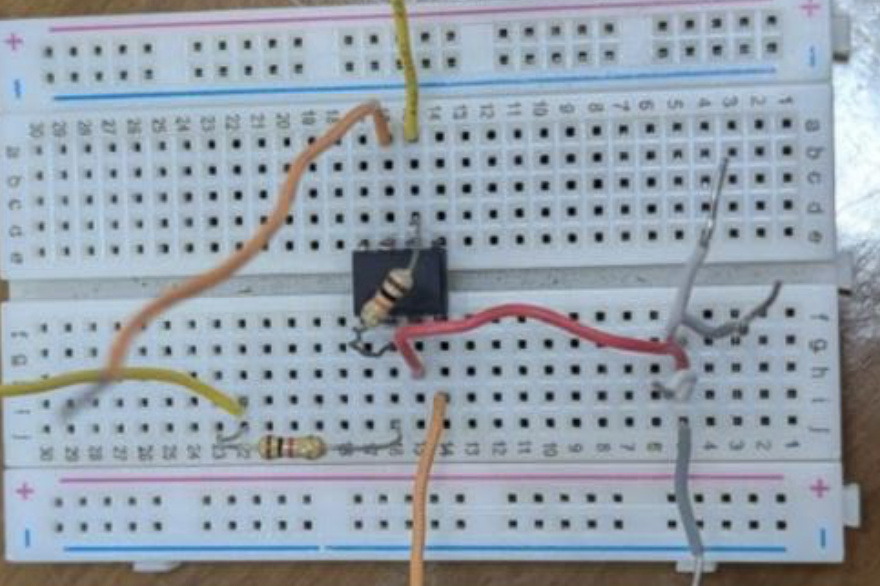
\includegraphics[width=0.7\linewidth]{figures/exp_1_step1.png}
        \caption{反向相放大器之麵包板架設圖}
        \label{fig:exp_1_step1}
    \end{figure}
    \item 調整訊號產生器參數:$V_{in}$ 使用 1kHz、DC Offset = 0、震幅:0.1V之正弦波;並將其連接接好的電路,使用示波器測量其$V_{out}$。
    \item 將$V_{in}$往上調整,觀察$V_{out}$之震幅最大可達到多少
    \item 改變$V_{in}$頻率,觀察其在高頻與低頻的運作
    \item 將訊號改成三角波輸入並觀察其圖形
    \item 紀錄放大器的輸入阻抗和其增益
\end{enumerate}

\clearpage
\subsection{同相放大器}\label{subsec:step_2}
\hfill

\begin{enumerate}
    \item 連接電路如Fig.\ref{fig:noninvert}
    \begin{figure}[h]
        \centering
        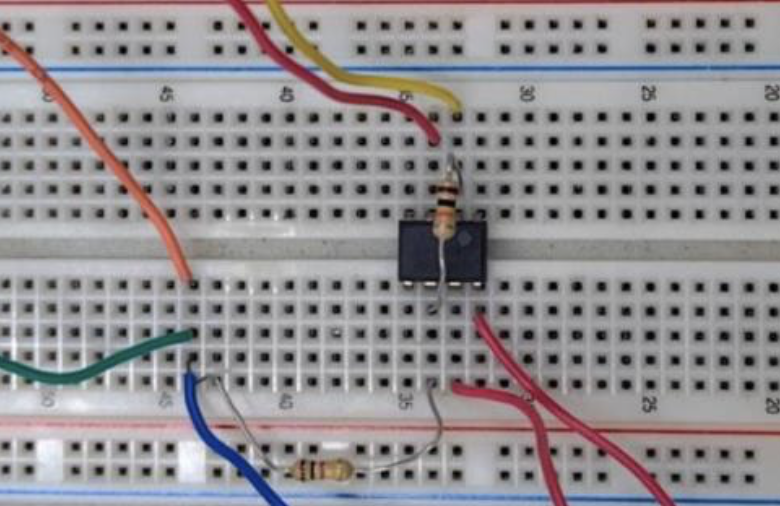
\includegraphics[width=0.7\linewidth]{figures/exp_2_step1.png}
        \caption{同向相放大器之麵包板架設圖}
        \label{fig:exp_2_step1}
    \end{figure}
    \item 重複Sec\ref{subsec:step_1}之步驟2.-6.
\end{enumerate}



% \clearpage
\subsection{隨耦器}
\hfill

\begin{enumerate}
    \item 連接電路如Fig.\ref{fig:follower}
    \begin{figure}[h]
        \centering
        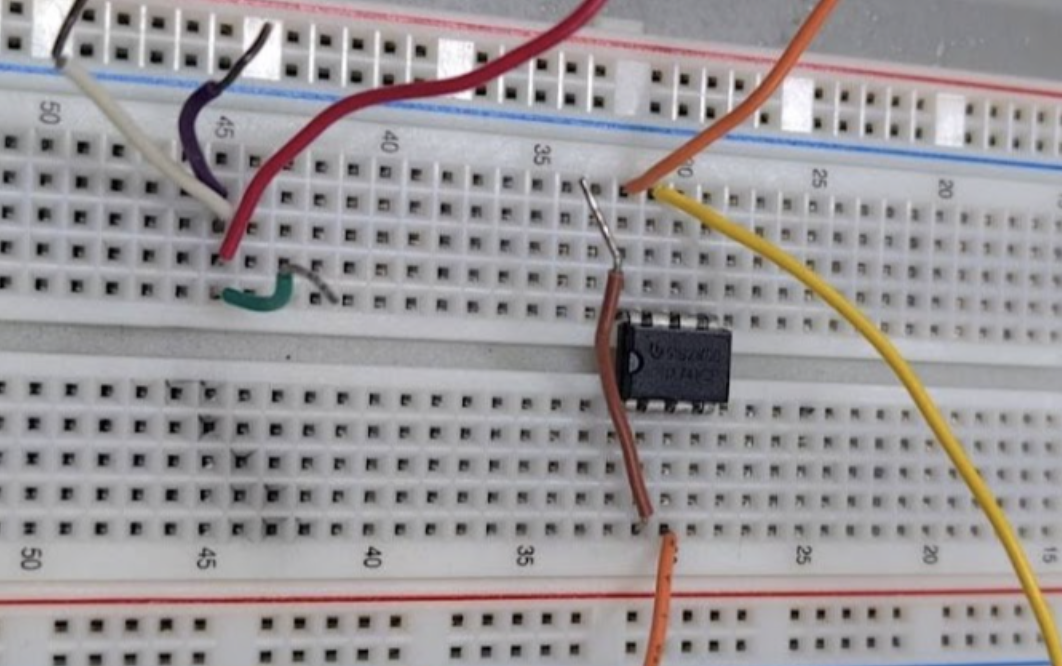
\includegraphics[width=0.7\linewidth]{figures/exp_3_step1.png}
        \caption{隨耦器之麵包板架設圖}
        \label{fig:exp_3_step1}
    \end{figure}
    \item 重複Sec\ref{subsec:step_1}之步驟2.-6.
\end{enumerate}

% \begin{center}
% \begin{tabular}{c c c c}
% $f_{in}$(Hz)    &   $V_{in}$(mV)    &   $V_{out}$(mV)   &   $f_{out}$(Hz)\\\hline\hline
% 1029    &   120.4   &   280.6   &   140.1   \\\hline
% \end{tabular}
% \end{center}

\section{實驗數據}\label{sec:result}
\hfill

\subsection{反向放大器}\label{subsec:result_1}
\hfill

\begin{figure}[h]
    \centering
    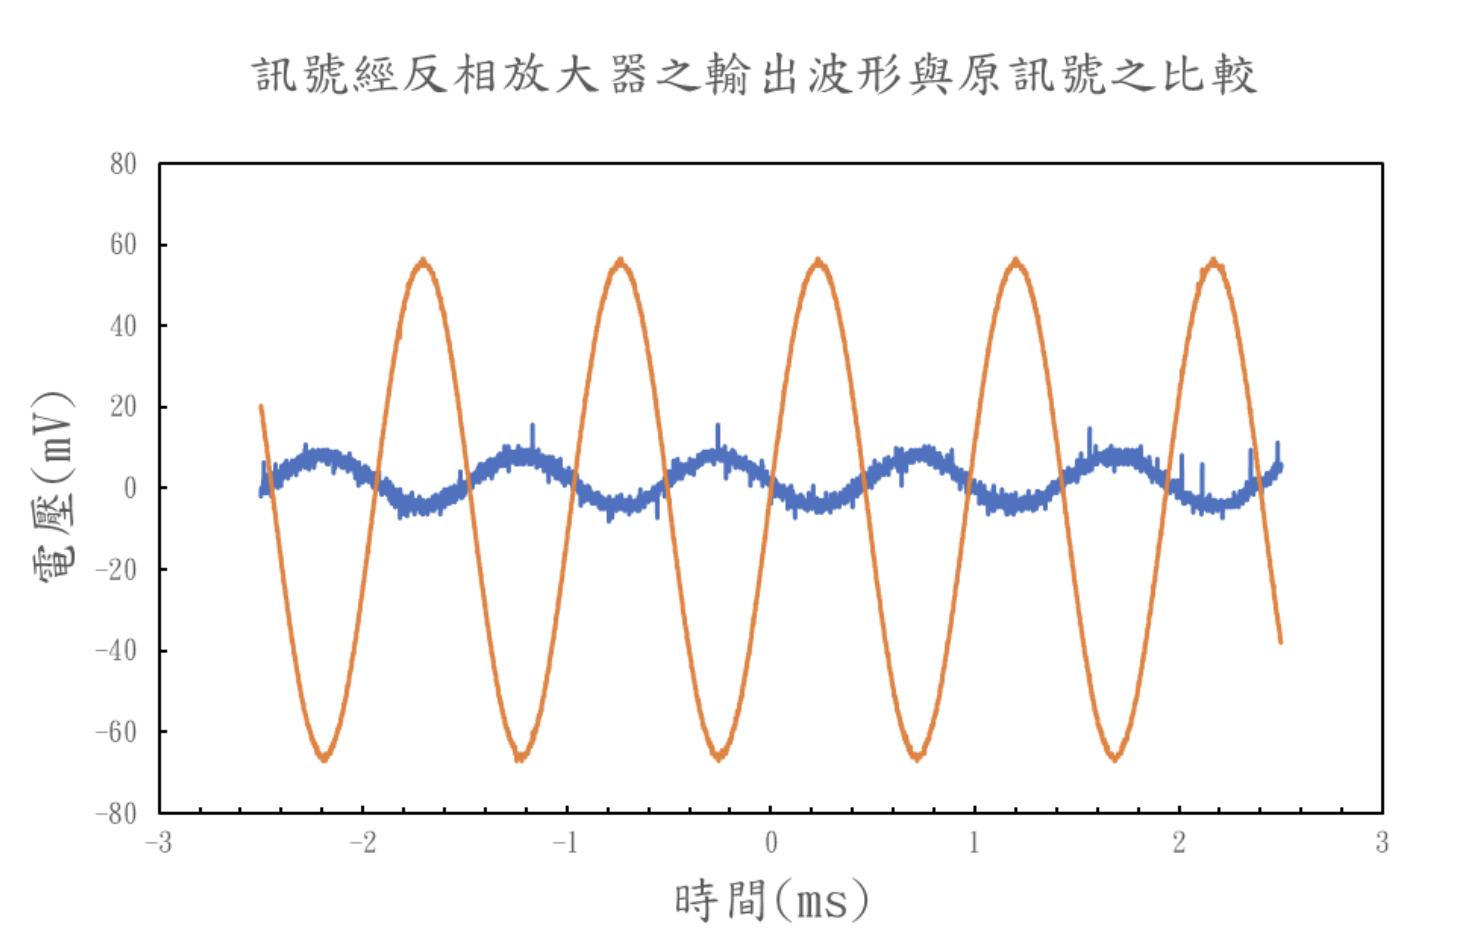
\includegraphics[width=0.7\linewidth]{figures/exp_1_result.png}
    \caption{反向放大器實驗數據(藍線為輸入訊號$V_{in}$,橘線為輸出訊號$V_{out}$)}
    \label{fig:exp_1_result}
\end{figure}

\begin{itemize}
    \item 實驗條件:$R_1$:942$\Omega$、$R_2$:9820$\Omega$、$f_{in}$:10.89Hz、$V_{in, AC}$:0.12V
    \item 實驗結果:$V_{out}$ = 119.6V
\end{itemize}

\subsection{同相放大器}\label{subsec:result_2}
\hfill

\begin{figure}[h]
    \centering
    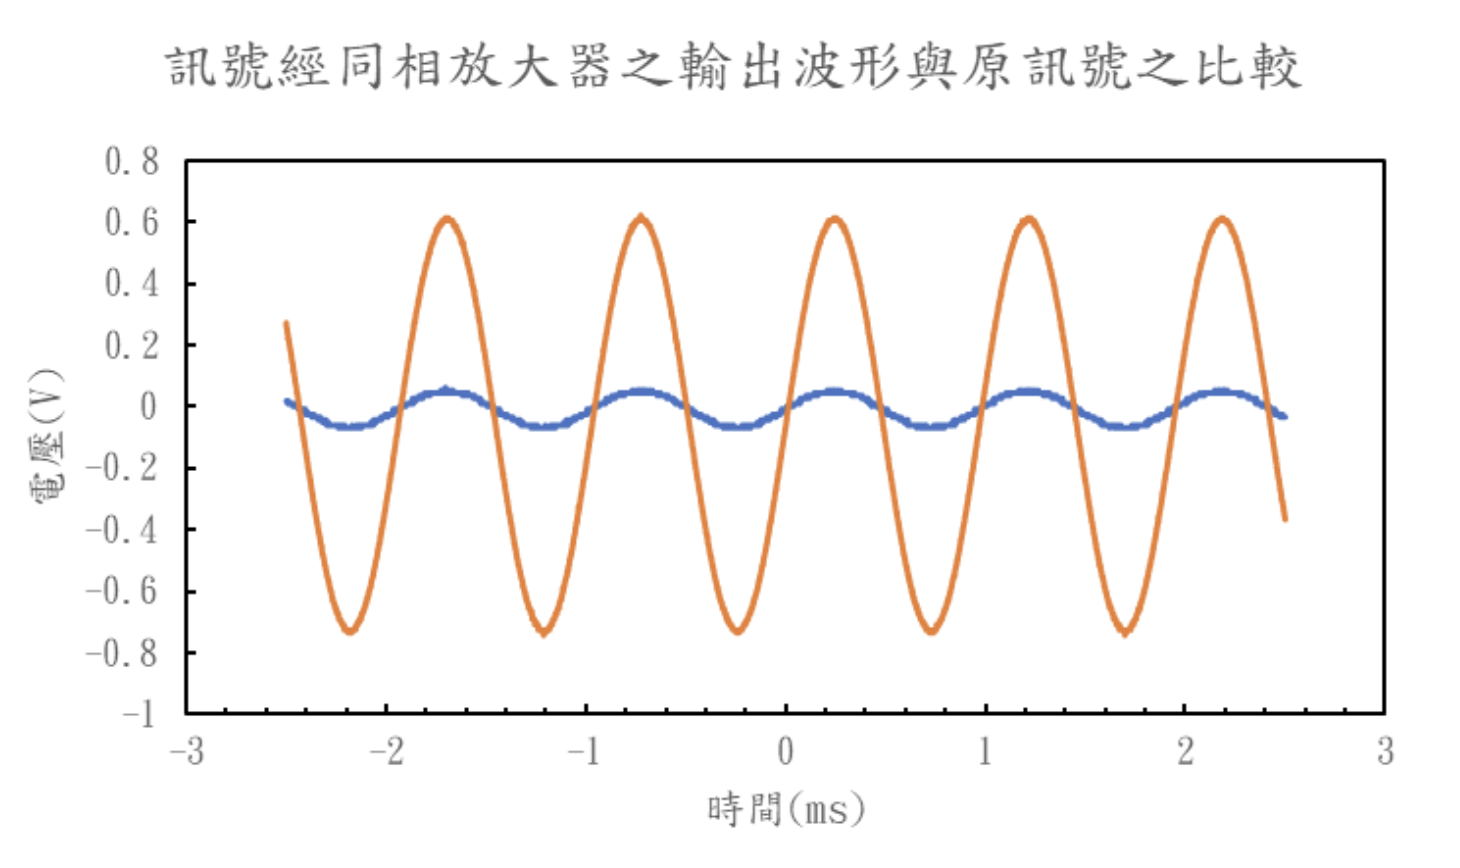
\includegraphics[width=0.7\linewidth]{figures/exp_2_result.png}
    \caption{正向放大器實驗數據(藍線為輸入訊號$V_{in}$,橘線為輸出訊號$V_{out}$)}
    \label{fig:exp_2_result}
\end{figure}

\begin{itemize}
    \item 實驗條件:$R_1$:970$\Omega$、$R_2$:9830$\Omega$、$f_{in}$:1034Hz、$V_{in, AC}$:0.105V
    \item 實驗結果:$V_{out}$ = 1.323V
\end{itemize}

\subsection{隨耦器}\label{subsec:result_3}
\hfill

\begin{figure}[h]
    \centering
    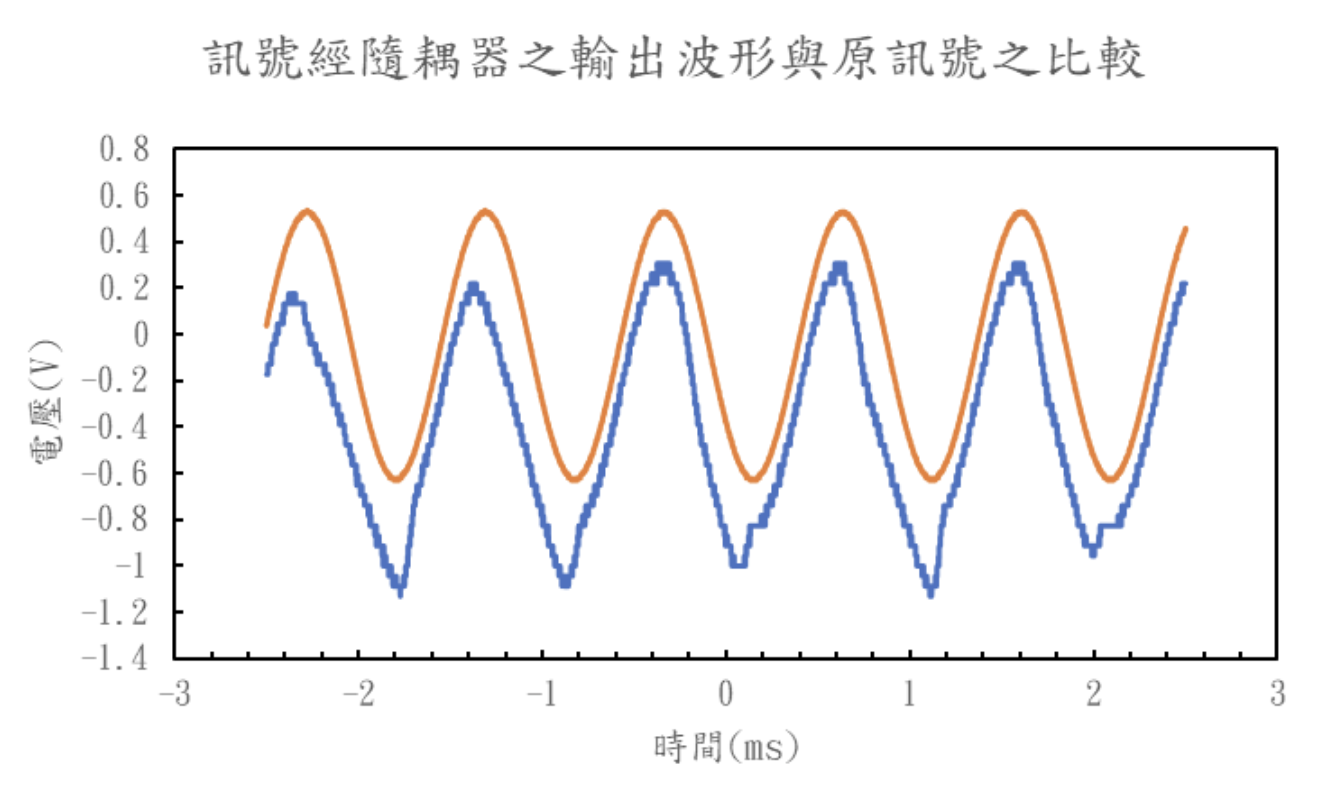
\includegraphics[width=0.7\linewidth]{figures/exp_3_result.png}
    \caption{隨耦器實驗數據(藍線為輸入訊號$V_{in}$,橘線為輸出訊號$V_{out}$)}
    \label{fig:exp_3_result}
\end{figure}

\begin{itemize}
    \item 實驗條件:$f_{in}$:1029Hz、$V_{in, AC}$:120.4V
    \item 實驗結果:$V_{out}$ = 280.6V、$f_{out}$:140.1H
\end{itemize}


\section{數據分析和問題討論}\label{sec:discussion}
\hfill

\subsection{反向放大器}\label{subsec:discussion_1}
\hfill

\begin{itemize}
    \item 從實驗結果之示波器圖形(Fig.\ref{fig:exp_1_result})來看,可知反相放大器會使輸出為輸入訊號相位相差180°的放大訊號;此與理論相符。
    \item 理論振幅使用Eq.\ref{eq:invert}計算:$V_{out, ideal}$ = 1.25 V,而我們所記錄的數據為$V_{out, exp}$ = 119.6V,約相差100倍。但由於已確認過線路、接線皆無錯誤,所以推測為記錄數據時將小數位數點錯,才造成100倍的誤差。而我們可以透過雙重確認的方式解決此問題,避免下次發生此類不應發生之疏失。 
\end{itemize}

\subsection{同相放大器}\label{subsec:discussion_2}
\hfill

\begin{itemize}
    \item 從實驗結果之示波器圖形(Fig.\ref{fig:exp_2_result})來看,可知同相放大器的輸入及輸出訊號同相位,並且訊號經過電路後將放大;此與理論相符。
    \item 理論振幅使用Eq.\ref{eq:noninvert}計算:$V_{out, ideal}$ = 1.169 V,而我們所記錄的數據為$V_{out, exp}$ = 1.323V,相比誤差值為13.2\%。此誤差可能因為接線沒有使電路好好連接,導致訊號雜亂,此時測量到的振幅即不精確;可透過將電路連接處再確實壓緊來改善。
\end{itemize}


\clearpage
\subsection{隨耦器}\label{subsec:discussion_3}
\hfill

從實驗結果之示波器圖形(Fig.\ref{fig:exp_3_result})來看,可知隨耦器並不因為放大器而產生放大效應,但會與原訊號有些許相位差;此與理論相符。

若我們需要減少相移,可透過以下方式: 
\begin{itemize}
    \item 選擇頻寬更高的運算放大器
    \item 減少輸出端之負載電容與負載阻抗
\end{itemize}

% \clearpage
\section{總結}
\hfill

此次實驗過程中遇到許多問題,花費不少時間嘗試排除,但由於時間有限加上助教有限,沒能完成所有實驗講義要求的成果。雖然沒能做出實驗講義要求的所有成果,我們仍能從實驗所得出之數據看出運算放大器的特色。 

\section{分工內容}
\hfill

\begin{itemize}
    \item 洪瑜:整理前言、數據分析
    \item 黃巧涵:PicoScope與訊號產生器操作
    \item 洪懌平:實驗操作接線
\end{itemize}

\section{參考文獻}
\hfill
\begin{enumerate}
    \item \url{https://shorturl.at/kj0ru}
\end{enumerate}


\end{CJK}
\end{document}
